\section{Pose Graph Optimization}
\label{sec:posegraph}
When the amount of registered frames increments, the accumulated error 
becomes visible. There is a drift respect to the real sensor trajectory. 
In order to deal with this problem, the most common approach is to use a pose graph 
optimization algorithm. 


Each pose of the sensor (rotation and translation) represents a node of the 
graph and each restriction between two poses represents an edge. The relative 
transformation between two poses is used as restriction.


The first pose of the graph can be arbitrary, in our case is set as the identity. Subsequent 
poses are determined by using relative transformations between pairs of frames, applying 
proposed technique. Each sensor frame corresponds to a graph pose. 

We have a non-linear least squares minimization problem that can be described by the following equation:

$$ F(x) = \sum\limits_{<i,j> \in C } e(x_i,x_j,z_{ij})^T \Omega_{ij} e(x_i,x_j,z_{ij}) $$

$$ x^* = \mathop{\rm argmin}_x F(x) \ ,$$

\noindent where $x=\{x_1,x_2,...,x_n\}$ and each $x_i$ represents a parameter block , $z_{i,j}$ and $\Omega_{ij}$ represents the mean  
 and the information matrix  of a constraint 
relating parameters $x_i$ and $x_j$. In our case $x_i$ corresponds to a sensor pose, $z_{ij}$ is the 
relative transformation between $i$-$esim$ and $j$-$esim$ sensor frame, it is not affected by the accumulated error 
because it is a direct measure between the two frames and $\Omega_{ij}$ is the weight or 
the confidence we give to the restriction. $\Omega_{ij}$ is a $7\times7$ diagonal matrix, containing on its diagonal the confidence ($\in [0,1]$) for each 
parameter of the transformation. 

Poses and relative transformations are represented by a $7\times1$ vector containing a translation vector
 and a normalized quaternion for the rotation:

$$ \begin{bmatrix} tx & ty & tz & qx & qy & qz & qw \end{bmatrix} ^T \ .$$



Then $e_{ij}$ is an error vector ($7\times1$) defined as follows:

$$
e(x_i,x_j,z_{ij}) = z_{ij} - \hat{z_{ij}} \ ,
$$

\noindent where $\hat{z_{ij}}$ is the relative transformation between $x_i$ and $x_j$ obtained directly from the pose graph, for this reason 
it is affected by the accumulated error.

We want to find a graph configuration (updating the poses $x=\{x_1,x_2,...,x_n\}$), that reduces global error,
 correcting some poses in order to satisfy the restrictions.

This  non-linear least squares problem can be solved using 
methods such as for example Gauss-Newton or Levenberg-Marquard \cite{numericalOptBook}.

\begin{figure}[!h]
\begin{center}
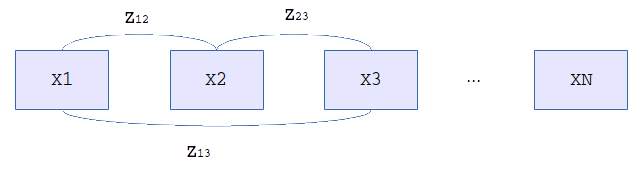
\includegraphics[scale=1.5]{images/graph_diagram2}
\caption{Graph of poses $(x_1,x_2,..)$ with constraints $(z_{12},z_{23},...)$ relating poses.}
\end{center}
\end{figure}

To simplify notation let: 

$$
e(x_i,x_j,z_{ij}) = e(x_i,x_j) = e_{ij}(x) \ ,
$$

\noindent we can approximate the previous function around one point:

\begin{equation}
\label{eq:errorAprox}
e_{ij}(x + \Delta x) \simeq e_{ij}(x) + J_{ij} \Delta x \ ,
\end{equation}

\noindent $J_{ij}$ is the Jacobian of the function evaluated in x. 


\begin{equation}
\label{eq:globalFunc}
F_{ij}(x + \Delta x) = e_{ij}(x + \Delta x)^T \Omega_{ij}  e_{ij}(x + \Delta x) \ .
\end{equation}

\noindent Replacing \ref{eq:errorAprox} in the global function:

\begin{equation}
\label{eq:globalFuncAprox}
F_{ij}(x + \Delta x) \simeq (e_{ij}(x) + J_{ij} \Delta x)^T \Omega_{ij}  (e_{ij}(x) + J_{ij} \Delta x) \ ,
\end{equation}

\begin{equation}
\label{eq:globalFuncAprox2}
 =  \underbrace{e_{ij}(x)^T \Omega_{ij} e_{ij}(x)}_{c_{ij}} + 2  \underbrace{e_{ij}(x)^T \Omega_{ij} J_{ij}}_{b_{ij}} \Delta x + \Delta x^T \underbrace{ J_{ij}^T  \Omega_{ij} J_{ij}}_{H_{ij}} \Delta x \ ,
\end{equation}

\begin{equation}
\label{eq:globalFuncAprox2}
 = c_{ij} + 2 b_{ij} \Delta x + \Delta x^T H_{ij} \Delta x \ ,
\end{equation}


\begin{equation}
F(x + \Delta x) =  \sum\limits_{<i,j> \in C } F_{ij}(x + \Delta x) \ ,
\end{equation}



\begin{equation}
\simeq  \sum\limits_{<i,j> \in C } c_{ij} + 2 b_{ij} \Delta x + \Delta x^T H_{ij} \Delta x \ ,
\end{equation}

\begin{equation}
\label{eq:lzn}
=   c + 2 b \Delta x + \Delta x^T H \Delta x \ ,
\end{equation}

\noindent where $c=\sum{c_{ij}}, b=\sum{b_{ij}}$ and $H=\sum{H_{ij}}$.

\noindent Then we want to know $\Delta x^*$, this is the correction to the nodes of the graph in order 
to have a minimum error. It can be obtained by solving the following linear system:

\begin{equation}
H \Delta x^* = -b \ .
\end{equation}

\noindent Having $\Delta x^*$ we can update the graph nodes:

\begin{equation}
x^* = x + \Delta x^* \ .
\end{equation}

The Gauss-Newton algorithm applies the linearization \ref{eq:lzn}, solves the linear system and uses the result as input of next iteration.

The Levenber-Marquardt (LM) is a nonlinear variant of the Gauss-Newton algorithm that introduces a
damping factor and backup actions to control the convergence:

\begin{equation}
(H + \lambda I) \Delta x^* = -b \ .
\end{equation}

\noindent The $\lambda$ factor controls the size of $ \Delta x^*$. Allowing changing it according to the error between the iterations.
 
The approach assumes that the spaces of parameters $x$ is Euclidean. However, this is not the case for the quaternion, 
in consequence it is necessary to apply the concept of manifold.


\subsection{Least Squares on Manifold}

A manifold is a topology space that is locally euclidean. In other words, each point has a neighborhood that is 
homeomorphic to the euclidean space. The manifold is not necessarily euclidean on a global scale, but can be seen 
as euclidean in a local scale \cite{manifold}.

The translation component of the parameters vector forms a euclidean space, but the rotation component does not.
In order to affront this problem the error minimization is applied on a manifold. The rotation is represented as a 
quaternion to avoid the singularities of use Euler angles (gimbal lock), but using a quaternion we have one extra 
dimension. Because a 3D rotation can be represented with three numbers and a quaternion has four. Applying the 
minimization using an overparametrized representation can lead to errors.

An alternative idea is to consider the underlying space as a manifold
and to define an operator $\boxplus$ that maps a local variation
$\Delta x$ in the Euclidean space to a variation on the manifold, $\Delta x \mapsto x + \Delta x$. 
Mathematical details can be found in \cite{hertzberg08}. The local variation is encoded using a minimal 
representation, the axis part of the quaternion $(q_i,q_j,q_k)$. The operator $\boxplus$ converts the 
resulting transformation to a full quaternion.

In order to define this operator, first lets define a composition operator $\oplus$:

$$
x_i \oplus x_j = \begin{bmatrix} t_i + q_i(t_j) \\ q_i \cdot q_j \end{bmatrix} \ ,
$$

\noindent where $q_i(t_j)$ is the vector resulting from applying rotation represented by $q_i$ to vector $t_j$ and 
$q_i \cdot q_j$ is the standard quaternion multiplication.

Then the operator $\boxplus$ is defined as follows:

$$
x_i \boxplus \Delta x_i = x_i \oplus \begin{bmatrix} \Delta t_i \\ \Delta q_i \\ \sqrt{1-||\Delta q_i||}  \end{bmatrix} \ .
$$

Note that $\Delta q_i$ contains only axis part of the quaternion.

Using this operator a new error function can be defined:

\begin{equation}
\begin{aligned}
\hat{e}_{ij}(\Delta x_i,\Delta x_j) &= e(x_i \boxplus \Delta x_i,x_j \boxplus \Delta x_j) \\
&= e_{ij}(x \boxplus \Delta x) \approx e_{ij} + \hat{J}_{ij} \Delta x \ ,
\end{aligned}
\end{equation}

\noindent where the Jacobian $\hat{J}_{ij}$ can be expressed as:

$$
\hat{J}_{ij} = \frac{\partial{e_{ij}(x \boxplus \Delta x)}}{\partial{\Delta x}} \bigg|_{\Delta x=0}
$$


G2o \cite{g2o} is a library that contains non linear error functions optimization 
algorithms for graphs and is widely used in registration algorithms. 

The poses where optimized using this library and specifically the 
Levenber-Marquardt algorithm.

Correction of the poses with this technique allows spreading error among the different nodes and reduces drift. The result 
will depend on the quality of the graph. A detailed explanation of this method is found in \cite{g2o}.

\subsection{Loop Closure}

When the sensor visits the same region at different times, for example following 
a circular trajectory. A restriction between two non-consecutive frames can be 
added to the graph. In the case of a circular trajectory, the accumulated error 
is very noticeable when the initial and the final frame are connected. Adding a 
restriction between this two frames to the graph allows adjusting 
the position of all poses in order to reduce the accumulated error. Loop Closure is 
a restriction between two non-consecutive poses.


\begin{figure}[!h]
\begin{center}
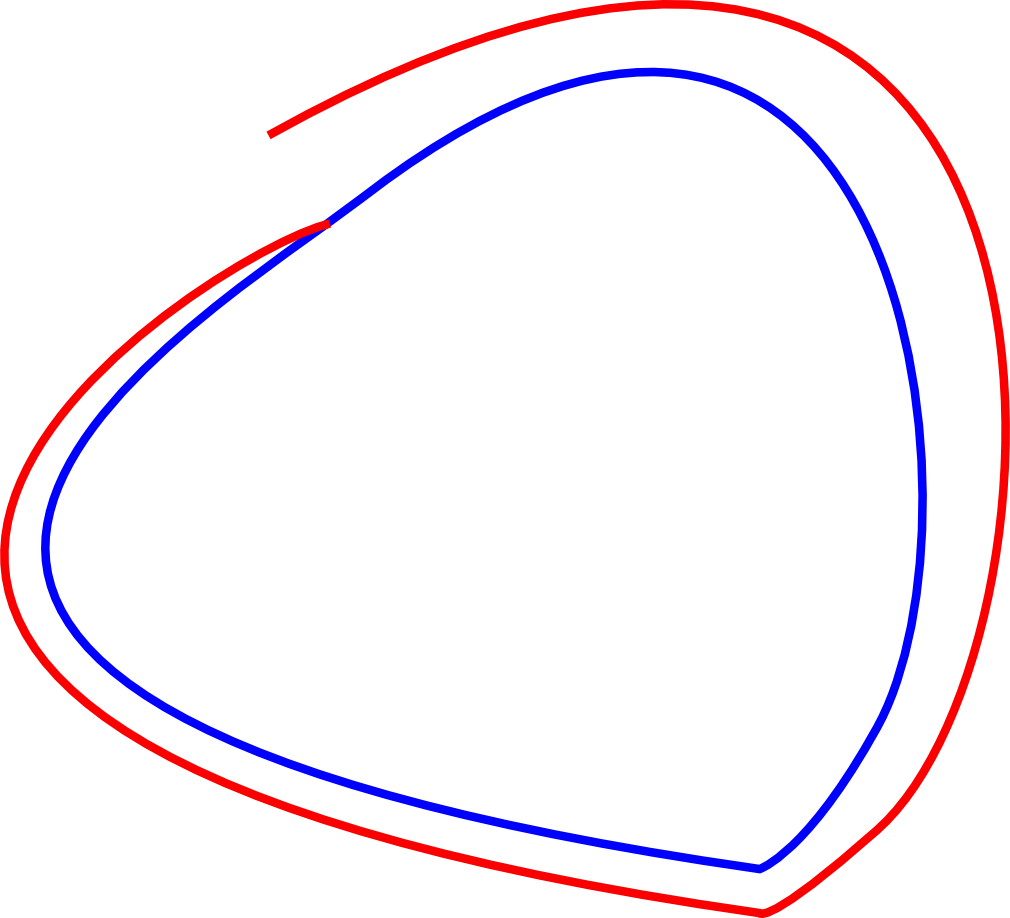
\includegraphics[scale=0.35]{images/drift}
\caption{Example of drift from real trajectory. Blue color: real camera trajectory, red color: estimation of trajectory with accumulated error.}
\end{center}
\end{figure}

\begin{figure}[!h]
\begin{center}
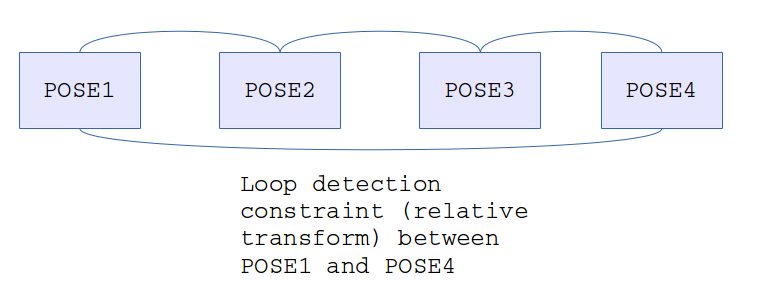
\includegraphics[scale=0.65]{images/loop_detection}
\caption{Example of loop closure constraint.}
\end{center}
\end{figure}

\subsubsection{Loop Detection}

In order to add loop closure constraints it is necessary to detect areas of the scene 
 that where previously visited. For this, images that have close euclidean distance between 
their corresponding poses are examined looking for similarities.

In order to detect previously visited areas of the scene SURF \cite{Bay06surf} feature detector 
is used. SURF keypoints are calculated and then the descriptors for each keypoint are obtained for 
each image.

 Then  the images are compared, using the difference between SURF descriptors.   

